% L2OALM: self-supervised primal-dual learning (PDL) with an augmented Lagrangian.
%
% Two proxies, x-hat(p) and lambda-hat(p). In the primal phase the dual proxy is
% frozen and the primal proxy minimizes the augmented Lagrangian (B2). In the
% dual phase the primal proxy is frozen and the dual proxy is regressed (B5)
% onto the multiplier step (B4) computed from a frozen copy lambda^k of itself.
% The outer iteration of Algorithm 1 alternates the phases and updates the
% penalty rho (B7). Notation and equation numbers follow docs/src/theory.md
% (box rows l <= c(x; p) <= u, one signed multiplier per row). The layout
% follows the primal-dual learning diagram of the author's website.
%
% Build: make -C docs/src/assets/diagrams/src
%   pdflatex -jobname=l2oalm--primal-dual alm.tex          -> wide layout
%   pdflatex -jobname=l2oalm--primal-dual-compact alm.tex  -> narrow layout
\documentclass[tikz,border=4pt]{standalone}
% Shared style of the LearningToOptimize diagrams: the palette, lane frames, cards,
% chips and glyphs of the paper-style TikZ figures (the same visual system as the
% PortfolioOpt.jl and DecisionRules.jl figures). Each figure \input's this file.
\usepackage{amsmath,amssymb,bm}
\usepackage[T1]{fontenc}
\usepackage[scaled=0.92]{helvet}
\renewcommand{\familydefault}{\sfdefault}
\usetikzlibrary{arrows.meta,shapes.geometric,shapes.symbols,calc,positioning,decorations.pathreplacing}

\definecolor{dTeal}{HTML}{1A9AA0}
\definecolor{dTealLine}{HTML}{3FB3B8}
\definecolor{dNavy}{HTML}{3F4C8C}
\definecolor{dInk}{HTML}{1E2235}
\definecolor{dRed}{HTML}{E4573D}
\definecolor{dCoral}{HTML}{E2765A}
\definecolor{dOrange}{HTML}{F4A93B}
\definecolor{dPeach}{HTML}{FBD9AC}
\definecolor{dPanel}{HTML}{EEF0F2}
\definecolor{dGray}{HTML}{8A90A0}
\definecolor{dNode}{HTML}{14A3A8}
\definecolor{dShadow}{HTML}{D5DAE3}

% \ifcompact is true when the job name ends in "-compact" (narrow layout).
\newif\ifcompact
\ifnum\pdfmatch{-compact$}{\jobname}=1 \compacttrue\fi

\tikzset{
  >={Stealth[length=5pt,width=4pt]},
  every node/.style={text=dInk},
  title/.style={anchor=west,font=\small,inner sep=0pt},
  head/.style={font=\small\bfseries,text=dNavy},
  note/.style={font=\itshape\footnotesize,text=dNavy},
  dnote/.style={font=\itshape\footnotesize,text=dCoral},
  code/.style={font=\ttfamily\footnotesize,text=dNavy},
  store/.style={cylinder,shape border rotate=90,aspect=0.28,fill=dPeach,draw=dOrange,
                line width=0.7pt,minimum width=0.95cm,minimum height=1.2cm,font=\normalsize},
  dia/.style={diamond,fill=dOrange,draw=none,minimum size=0.9cm,inner sep=0pt,aspect=1,
              font=\normalsize},
  lnode/.style={circle,fill=dRed,draw=none,minimum size=0.66cm,inner sep=1pt,
                text=white,font=\normalsize},
  card/.style={rectangle,rounded corners=4pt,fill=white,draw=dShadow,line width=0.6pt},
  sheet/.style={rectangle,rounded corners=3pt,fill=dPanel,draw=dShadow,line width=0.6pt},
  chip/.style={rectangle,rounded corners=3pt,fill=dPanel,draw=none,font=\small,
               inner xsep=4pt,inner ysep=3pt},
  ochip/.style={chip,fill=white,draw=dGray,dashed,line width=0.6pt},
  pchip/.style={chip,fill=white,draw=dGray!70,dashed,line width=0.5pt,text=dGray},
  fwd/.style={->,dTealLine,line width=0.8pt},
  tgt/.style={->,dOrange,line width=0.9pt},
  dual/.style={->,dCoral,dashed,line width=0.9pt},
  dep/.style={->,dTealLine,line width=0.8pt},
  pdep/.style={->,dGray,dashed,line width=0.7pt},
  nn/.style={circle,minimum size=0.26cm,inner sep=0pt,draw=dInk!70,line width=0.35pt},
}

% Lane frame in the paper style: two shadow copies behind a teal rounded frame.
\newcommand{\lane}[4]{% #1 x0, #2 y0, #3 x1, #4 y1
  \foreach \o/\c in {0.16/dShadow!60,0.08/dShadow}
    \draw[\c,fill=white,rounded corners=5pt,line width=0.6pt]
      (#1+\o,#2-\o) rectangle (#3+\o,#4-\o);
  \draw[dTealLine,fill=white,rounded corners=5pt,line width=0.9pt] (#1,#2) rectangle (#3,#4);}

% Plain card frame (no shadow copies), for problems and losses.
\newcommand{\cardbox}[4]{\draw[dShadow,fill=white,rounded corners=4pt,line width=0.6pt] (#1,#2) rectangle (#3,#4);}

% Network glyph on one sheet. #1 = centre, #2 = name prefix, #3 = number of stacked
% sheets behind (0, 1 or 2).
\newcommand{\net}[3]{%
  \begin{scope}[shift={(#1)}]
    \ifnum#3>1 \node[sheet,minimum width=1.9cm,minimum height=1.8cm] at (0.30,0.22) {};\fi
    \ifnum#3>0 \node[sheet,minimum width=1.9cm,minimum height=1.8cm] at (0.15,0.11) {};\fi
    \node[sheet,minimum width=1.9cm,minimum height=1.8cm,fill=white] (#2sheet) at (0,0) {};
    \foreach \y [count=\i] in {0.36,0,-0.36} \node[nn,fill=dGray!45] (#2in\i) at (-0.64,\y) {};
    \foreach \y [count=\i] in {0.58,0.29,0,-0.29,-0.58} \node[nn,fill=dNode] (#2ha\i) at (-0.21,\y) {};
    \foreach \y [count=\i] in {0.44,0.15,-0.15,-0.44} \node[nn,fill=dNode] (#2hb\i) at (0.21,\y) {};
    \node[nn,fill=dOrange] (#2out) at (0.64,0) {};
    \foreach \a in {1,...,3} \foreach \b in {1,...,5} \draw[dGray!60,line width=0.2pt] (#2in\a) -- (#2ha\b);
    \foreach \a in {1,...,5} \foreach \b in {1,...,4} \draw[dGray!60,line width=0.2pt] (#2ha\a) -- (#2hb\b);
    \foreach \a in {1,...,4} \draw[dGray!60,line width=0.2pt] (#2hb\a) -- (#2out);
  \end{scope}}

% Jacobian mask glyph: an n x d grid with a few entries selected. #1 = centre.
\newcommand{\maskgrid}[1]{%
  \begin{scope}[shift={(#1)}]
    \foreach \i in {0,...,4} \foreach \j in {0,...,3}
      \draw[dShadow,fill=white,line width=0.4pt] (\j*0.2-0.4,-\i*0.2+0.5) rectangle ++(0.2,-0.2);
    \foreach \i/\j in {0/1,1/3,2/0,3/2,4/1}
      \draw[dOrange,fill=dOrange,line width=0.4pt] (\j*0.2-0.4,-\i*0.2+0.5) rectangle ++(0.2,-0.2);
  \end{scope}}

% Code names inside italic notes stay upright.
\newcommand{\cmd}[1]{{\upshape\ttfamily #1}}

% Software-architecture helpers: package cards, type chips and chip rows.
\tikzset{
  pkg/.style={rectangle,rounded corners=4pt,fill=white,draw=dShadow,line width=0.6pt,
              align=center,inner xsep=5pt,inner ysep=4pt,font=\footnotesize},
  pkgcore/.style={pkg,draw=dTealLine,line width=0.9pt},
  pkgplan/.style={pkg,draw=dGray,dashed,text=dGray},
  tchip/.style={chip,font=\ttfamily\footnotesize,inner xsep=3pt,inner ysep=2.5pt},
  tplan/.style={tchip,fill=white,draw=dGray,dashed,line width=0.5pt,text=dGray},
  absname/.style={anchor=west,font=\ttfamily\footnotesize,text=dNavy,inner sep=1pt},
}
% \chiprow{x}{y}{style}{A,B,C}: chips left to right from (x,y), anchored west.
\newcommand{\chiprow}[4]{%
  \coordinate (cr@next) at (#1,#2);
  \foreach \t in {#4} {%
    \node[#3,anchor=west] (cr@last) at (cr@next) {\t};
    \coordinate (cr@next) at ($(cr@last.east)+(0.12,0)$);}}


\newcommand{\Lp}{%
  $\begin{aligned}
    \mathcal{L}_p=\;& s\,f(\hat x)+\textstyle\sum_i\big(\lambda_i^+(c_i-u_i)+\lambda_i^-(l_i-c_i)\big)\\
    &+\tfrac{\rho}{2}\textstyle\sum_i v_i^2\;\;\text{(B2)}
  \end{aligned}$}
\newcommand{\Lpnote}{$v_i=\max(l_i-c_i,0)+\max(c_i-u_i,0)$;\; batch mean}
\newcommand{\Ld}{$\mathcal{L}_d=\big\|(\hat\lambda-t)_{\mathcal{G}}\big\|_\varepsilon+\big\|(\hat\lambda-t)_{\mathcal{H}}\big\|_\varepsilon$\;\;(B5)}
\newcommand{\target}{$t=\Pi_M\big(\lambda^k+\rho\,\sigma(\hat x,\lambda^k)\big)$\;\;(B4)}
\newcommand{\sigmadef}{$\sigma(x,\lambda)=c(x)-\Pi_{[l,u]}\big(c(x)+\lambda/\rho\big)$}
\newcommand{\steps}[1]{(i) primal phase on $\mathcal{L}_p$#1(ii) violation $v_k$ (8)#1(iii) copy $\lambda^k$#1(iv) dual phase on $\mathcal{L}_d$#1(v) $\rho\leftarrow\min(\alpha\rho,\rho_{\max})$ if $v_k>\tau\,v_{k-1}$ (B7)}

\begin{document}
\ifcompact
% ============================ narrow (phone) layout ============================
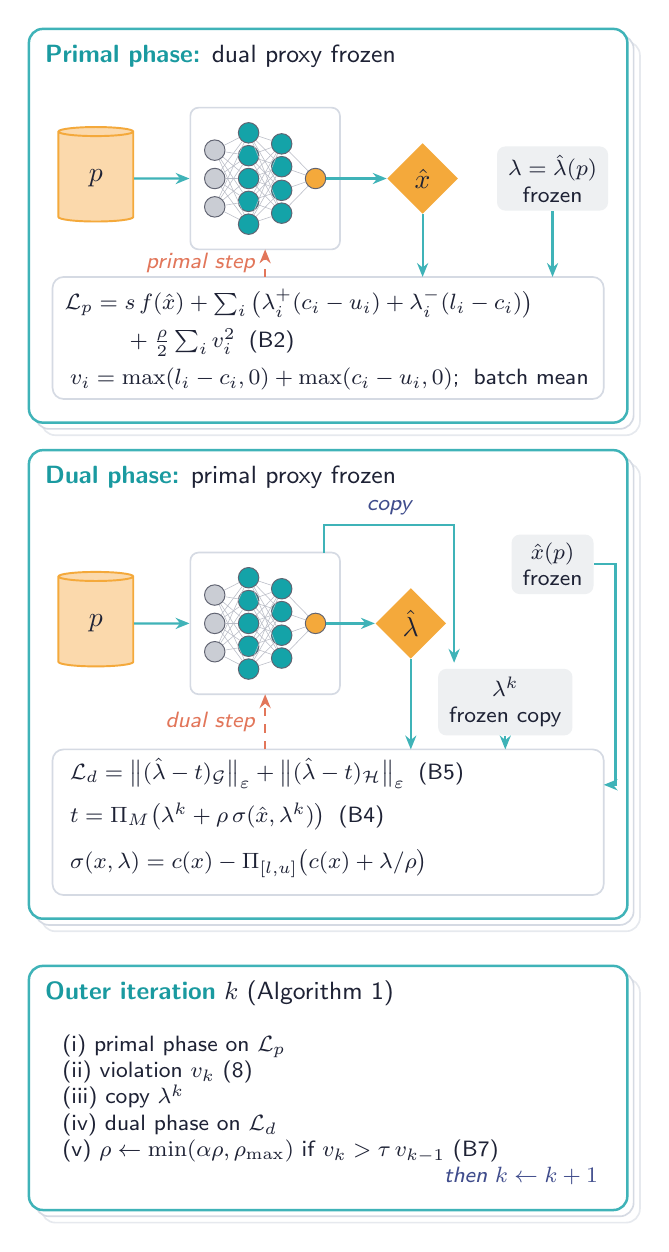
\begin{tikzpicture}
  % ---- primal phase ----
  \lane{0}{10.0}{7.6}{15.0}
  \node[title] at (0.2,14.65) {\textcolor{dTeal}{\bfseries Primal phase:} dual proxy frozen};
  \node[store] (p) at (0.85,13.1) {$p$};
  \net{3.0,13.1}{pp}{0}
  \draw[fwd] (p.east) -- (ppsheet.west);
  \node[dia] (xh) at (5.0,13.1) {$\hat x$};
  \draw[fwd] (ppout.east) -- (xh.west);
  \node[chip,align=center,font=\footnotesize] (lf) at (6.65,13.1) {$\lambda=\hat\lambda(p)$\\frozen};
  \cardbox{0.3}{10.3}{7.3}{11.85}
  \node[anchor=north west,font=\footnotesize,inner sep=0pt] at (0.45,11.7) {\Lp};
  \node[font=\footnotesize,anchor=west] at (0.4,10.55) {\Lpnote};
  \draw[fwd] (xh.south) -- (5.0,11.85);
  \draw[fwd] (lf.south) -- (6.65,11.85);
  \draw[dual] (3.0,11.85) -- node[left,dnote] {primal step} (3.0,12.2);
  % ---- dual phase ----
  \lane{0}{3.7}{7.6}{9.65}
  \node[title] at (0.2,9.3) {\textcolor{dTeal}{\bfseries Dual phase:} primal proxy frozen};
  \node[store] (p2) at (0.85,7.45) {$p$};
  \net{3.0,7.45}{dp}{0}
  \draw[fwd] (p2.east) -- (dpsheet.west);
  \node[dia] (lh) at (4.85,7.45) {$\hat\lambda$};
  \draw[fwd] (dpout.east) -- (lh.west);
  \node[chip,align=center,font=\footnotesize] (lk) at (6.05,6.45) {$\lambda^k$\\frozen copy};
  \node[chip,align=center,font=\footnotesize] (xf) at (6.65,8.2) {$\hat x(p)$\\frozen};
  \draw[fwd] (3.75,8.35) |- node[pos=0.75,above,font=\footnotesize\itshape,text=dNavy] {copy} (5.4,8.7) -- (5.4,6.95);
  \cardbox{0.3}{4.0}{7.3}{5.85}
  \node[font=\footnotesize,anchor=west] at (0.4,5.55) {\Ld};
  \node[font=\footnotesize,anchor=west] at (0.4,5.0) {\target};
  \node[font=\footnotesize,anchor=west] at (0.4,4.4) {\sigmadef};
  \draw[fwd] (lh.south) -- (4.85,5.85);
  \draw[fwd] (lk.south) -- (6.05,5.85);
  \draw[fwd] (xf.east) -- (7.45,8.2) -- (7.45,5.4) -- (7.3,5.4);
  \draw[dual] (3.0,5.85) -- node[left,dnote] {dual step} (3.0,6.55);
  % ---- outer iteration ----
  \lane{0}{0}{7.6}{3.1}
  \node[title] at (0.2,2.75) {\textcolor{dTeal}{\bfseries Outer iteration} $k$ (Algorithm 1)};
  \node[font=\footnotesize,anchor=north west,align=left] at (0.3,2.35) {\steps{\\}};
  \node[note,anchor=south east] at (7.35,0.2) {then $k\leftarrow k+1$};
\end{tikzpicture}
\else
% =============================== wide layout ===================================
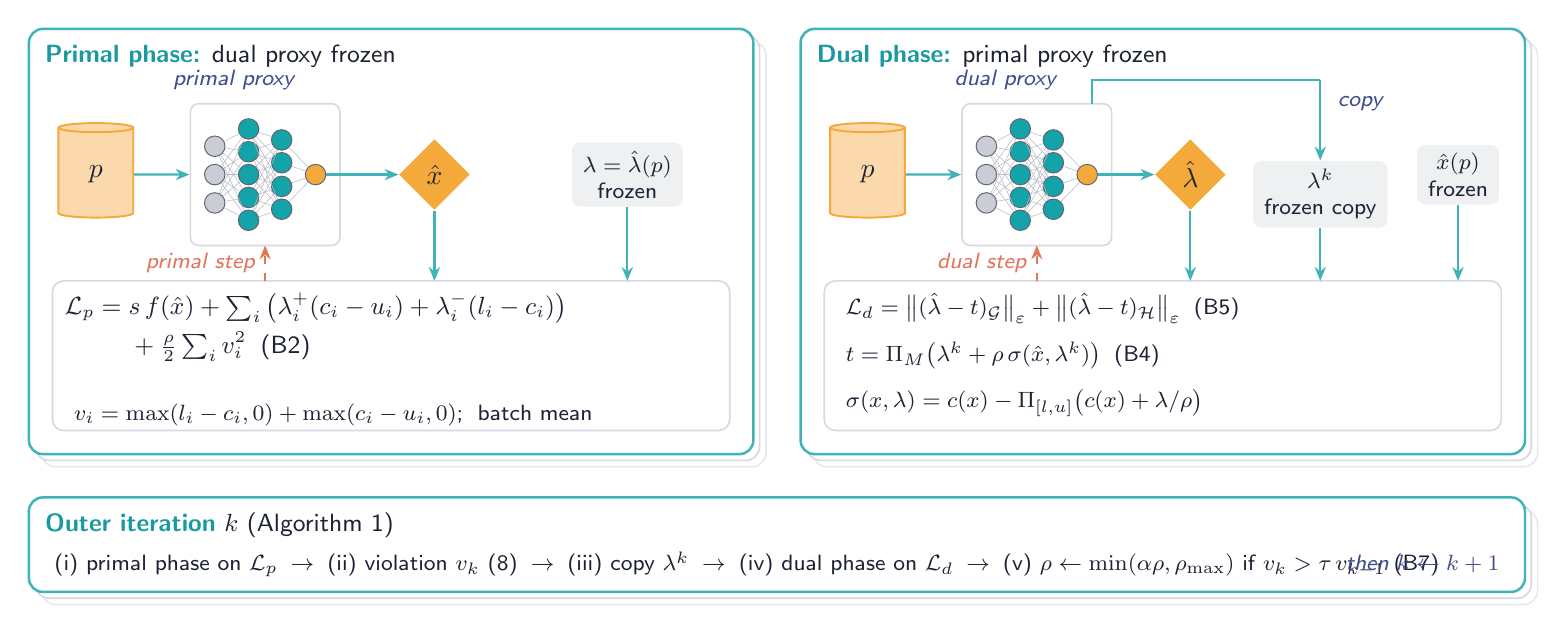
\begin{tikzpicture}
  % ---- primal phase (left) ----
  \lane{0}{0}{9.2}{5.4}
  \node[title] at (0.2,5.05) {\textcolor{dTeal}{\bfseries Primal phase:} \textcolor{dInk}{dual proxy frozen}};
  \node[store] (p) at (0.85,3.55) {$p$};
  \net{3.0,3.55}{pp}{0}
  \node[note] at (2.6,4.75) {primal proxy};
  \draw[fwd] (p.east) -- (ppsheet.west);
  \node[dia] (xh) at (5.15,3.55) {$\hat x$};
  \draw[fwd] (ppout.east) -- (xh.west);
  \node[chip,align=center,font=\footnotesize] (lf) at (7.6,3.55) {$\lambda=\hat\lambda(p)$\\frozen};
  \cardbox{0.3}{0.3}{8.9}{2.2}
  \node[anchor=north west,font=\small,inner sep=0pt] at (0.45,2.05) {\Lp};
  \node[font=\footnotesize,anchor=west] at (0.45,0.5) {\Lpnote};
  \draw[fwd] (xh.south) -- (5.15,2.2);
  \draw[fwd] (lf.south) -- (7.6,2.2);
  \draw[dual] (3.0,2.2) -- node[left,dnote] {primal step} (3.0,2.65);

  % ---- dual phase (right) ----
  \lane{9.8}{0}{19.0}{5.4}
  \node[title] at (10.0,5.05) {\textcolor{dTeal}{\bfseries Dual phase:} \textcolor{dInk}{primal proxy frozen}};
  \node[store] (p2) at (10.65,3.55) {$p$};
  \net{12.8,3.55}{dp}{0}
  \node[note] at (12.4,4.75) {dual proxy};
  \draw[fwd] (p2.east) -- (dpsheet.west);
  \node[dia] (lh) at (14.75,3.55) {$\hat\lambda$};
  \draw[fwd] (dpout.east) -- (lh.west);
  \node[chip,align=center,font=\footnotesize] (lk) at (16.4,3.3) {$\lambda^k$\\frozen copy};
  \node[chip,align=center,font=\footnotesize] (xf) at (18.15,3.55) {$\hat x(p)$\\frozen};
  \draw[fwd] (16.4,4.75) -- (lk.north);
  \node[note,anchor=west] at (16.5,4.45) {copy};
  \cardbox{10.1}{0.3}{18.7}{2.2}
  \node[font=\footnotesize,anchor=west] at (10.25,1.85) {\Ld};
  \node[font=\footnotesize,anchor=west] at (10.25,1.25) {\target};
  \node[font=\footnotesize,anchor=west] at (10.25,0.65) {\sigmadef};
  \draw[fwd] (lh.south) -- (14.75,2.2);
  \draw[fwd] (lk.south) -- (16.4,2.2);
  \draw[fwd] (xf.south) -- (18.15,2.2);
  \draw[dual] (12.8,2.2) -- node[left,dnote] {dual step} (12.8,2.65);
  \draw[dTealLine,line width=0.8pt] (13.5,4.45) -- (13.5,4.75) -- (16.4,4.75);

  % ---- outer iteration (bottom) ----
  \lane{0}{-1.75}{19.0}{-0.55}
  \node[title] at (0.2,-0.9) {\textcolor{dTeal}{\bfseries Outer iteration} $k$ \textcolor{dInk}{(Algorithm 1)}};
  \node[font=\footnotesize,anchor=west] at (0.2,-1.4) {\steps{\;\;$\rightarrow$\;\;}};
  \node[note,anchor=east] at (18.8,-1.4) {then $k\leftarrow k+1$};
\end{tikzpicture}
\fi
\end{document}
